\documentclass[11pt]{article}

% --- Packages ---
\usepackage[utf8]{inputenc}
\usepackage[T1]{fontenc}
\usepackage{lmodern}
\usepackage[margin=1in]{geometry}
\usepackage{amsmath, amssymb, amsthm, mathtools}
\usepackage{listings}
\usepackage{xcolor}
\usepackage{hyperref}
\usepackage{cleveref}
\usepackage{tikz}

\crefname{theorem}{Theorem}{Theorems}
\Crefname{theorem}{Theorem}{Theorems}
\crefname{lemma}{Lemma}{Lemmas}
\Crefname{lemma}{Lemma}{Lemmas}
\crefname{proposition}{Proposition}{Propositions}
\Crefname{proposition}{Proposition}{Propositions}
\crefname{corollary}{Corollary}{Corollaries}
\Crefname{corollary}{Corollary}{Corollaries}
\crefname{definition}{Definition}{Definitions}
\Crefname{definition}{Definition}{Definitions}
\crefname{example}{Example}{Examples}
\Crefname{example}{Example}{Examples}
\crefname{remark}{Remark}{Remarks}
\Crefname{remark}{Remark}{Remarks}

% --- Theorem environments ---
\theoremstyle{plain}
\newtheorem{theorem}{Theorem}[section]
\newtheorem{lemma}[theorem]{Lemma}
\newtheorem{proposition}[theorem]{Proposition}
\newtheorem{corollary}[theorem]{Corollary}

\theoremstyle{definition}
\newtheorem{definition}[theorem]{Definition}
\newtheorem{example}[theorem]{Example}

\theoremstyle{remark}
\newtheorem{remark}[theorem]{Remark}

% --- Lean listing setup ---
\definecolor{leankeyword}{RGB}{0,0,180}
\definecolor{leancomment}{RGB}{100,100,100}
\definecolor{leanstring}{RGB}{160,0,0}
\definecolor{leanbg}{RGB}{248,248,248}

\lstdefinelanguage{lean}{
  morekeywords={
    theorem,lemma,definition,def,example,axiom,structure,inductive,class,instance,
    variable,variables,namespace,end,open,import,section,universe,universes,
    fun,let,in,if,then,else,match,with,do,return,have,show,by,from,this,
    suffices,calc,Type,Prop,Sort,Pi,forall,exists,
    where,deriving,abbrev,notation,infixl,infixr,prefix,postfix,mutual
  },
  sensitive=true,
  morecomment=[l]{--},
  morecomment=[s]{/-}{-/},
  morestring=[b]",
  literate=
    {α}{{$\alpha$}}1 {β}{{$\beta$}}1 {γ}{{$\gamma$}}1 {δ}{{$\delta$}}1
    {ε}{{$\varepsilon$}}1 {λ}{{$\lambda$}}1 {μ}{{$\mu$}}1 {σ}{{$\sigma$}}1
    {τ}{{$\tau$}}1 {φ}{{$\varphi$}}1 {ψ}{{$\psi$}}1 {ω}{{$\omega$}}1
    {Γ}{{$\Gamma$}}1 {Δ}{{$\Delta$}}1 {Σ}{{$\Sigma$}}1 {Π}{{$\Pi$}}1
    {ℕ}{{$\mathbb{N}$}}1 {ℤ}{{$\mathbb{Z}$}}1 {ℚ}{{$\mathbb{Q}$}}1
    {ℝ}{{$\mathbb{R}$}}1 {ℂ}{{$\mathbb{C}$}}1
    {→ₗ}{{$\to_{\ell}$}}1 {≃ₗ}{{$\simeq_{\ell}$}}1 {ₗ}{{$_{\ell}$}}1
    {→}{{$\to$}}1 {↦}{{$\mapsto$}}1 {⟶}{{$\longrightarrow$}}1
    {∀}{{$\forall$}}1 {∃}{{$\exists$}}1 {¬}{{$\neg$}}1
    {∧}{{$\wedge$}}1 {∨}{{$\vee$}}1 {↔}{{$\leftrightarrow$}}1
    {∣}{{$\mid$}}1
    {≤}{{$\leq$}}1 {≥}{{$\geq$}}1 {≠}{{$\neq$}}1 {≡}{{$\equiv$}}1
    {∈}{{$\in$}}1 {∉}{{$\notin$}}1 {⊆}{{$\subseteq$}}1 {⊂}{{$\subset$}}1
    {⧸}{{$/$}}1
    {∪}{{$\cup$}}1 {∩}{{$\cap$}}1 {∅}{{$\emptyset$}}1
    {⟨}{{$\langle$}}1 {⟩}{{$\rangle$}}1 {·}{{$\cdot$}}1 {∘}{{$\circ$}}1
}

\lstset{
  language=lean,
  basicstyle=\ttfamily\small,
  keywordstyle=\color{leankeyword}\bfseries,
  commentstyle=\color{leancomment}\itshape,
  stringstyle=\color{leanstring},
  backgroundcolor=\color{leanbg},
  frame=single,
  rulecolor=\color{black!20},
  showstringspaces=false,
  breaklines=true,
  breakatwhitespace=true,
  columns=fullflexible,
  keepspaces=true,
  numbers=left,
  numberstyle=\tiny\color{gray},
  numbersep=8pt,
  xleftmargin=2.5em,
  framexleftmargin=2em,
  captionpos=b,
}

% Shorthand for inline Lean code
\newcommand{\lean}[1]{\lstinline[language=lean]|#1|}

% --- Metadata ---
\title{ChainCert: Certified Simplicial Homology Computations in Lean Using Sage}
\author{Lucy Horowitz}
\date{May 16, 2026}

\begin{document}
\maketitle

\begin{abstract}
A short summary of what was formalized, why it matters, and the main results.
\end{abstract}

\section{Introduction}\label{sec:intro}
Interactive theorem provers (ITPs) like Lean are very good at checking proofs but not so good at computing. Computer algebra systems (CAS) like Sage are very good at computing but offer no formal guarantees on their answers. Large parts of modern mathematics already rely on CAS, and with recent rapid strides in autoformalization, more mathematics is formalized every day. There is still a critical gap, however, between ``what the CAS said'' and ``what we've formally proved'' if we want to use CAS results downstream in proofs. 

In theory it is possible to re-implement the necessary algorithms in Lean or prove that the implementation in Sage is correct, but this is difficult. Algorithms may be enormously complicated or rely on space-saving hacks for efficiency that Lean isn't able to take advantage of. Moreover, Lean isn't built for numerical work in the first place.

Another strategy to solve this problem is to let each system do what it is good at at build a concrete bridge between them. Instead of blindly trusting Sage's answer, we can modify what it outputs so that Lean is capable of checking the answer. The output is a \textit{certificate} of computation: a small amount of additional data that is sufficient for the verification of the result. This moves the trust boundary from all of Sage to Lean's typechecker. This general pattern of certificate-based CAS-Lean interaction follows Baanen et al. \cite{baanen}.

This project develops the paradigm for the concrete case of integral homology of a finite simplicial complex. Computing the homology groups is simple and well-understood: it takes nothing more than computing the boundary matrices, computing two Smith normal forms, and reading off the invariant factors. If you ask Sage to compute the homology groups of a simplicial complex it will just give you the Betti numbers and torsion coefficients, not any of the intermediate matrices. With just these numbers alone, it is not possible to check whether or not the answer is correct. We instead ask sage for a full certificate, including the Smith normal forms (which have their own certificates) and prove a theorem in Lean that this is sufficient to guarantee correctness of the computation. 

Homology is a useful first target for this kind of certificate-based bridge because the underlying linear algebra is concrete and well-understood, the certificates are small and easy to specify, while the workflow exposes every part of the interface between Sage and Lean, from serialization of ring elements to parsing structured output and constructing \lean{Expr}s.

The rest of the paper is structured as follows: \Cref{sec:background} reviews the mathematical background necessary for computing the homology groups of a simplicial complex using the SNF. It is short and self-contained beyond some basic facts and definitions in algebra and topology. \cref{sec:certificates} introduces the certificates we defined and proves their soundness. \cref{sec:theorems} collects the main verified ``bridge theorems'' connecting those certificates to Mathlib quotient objects. \cref{sec:tactics} describes the Lean tactics and commands that construct the certificates from Sage output. \cref{sec:examples} works through concrete examples. 


\section{Background}\label{sec:background}
\subsection{Smith Normal Form}
Let $R$ be a principal ideal domain. For the purposes of this project, we will always be dealing with the integers, but the results work more generally. 

\begin{definition}[Smith Normal Form]\label[definition]{def:snf}
    Let $A$ be an $n\times m$ matrix with entries in $R$. The \textbf{Smith normal form} of $A$ is a diagonal matrix $D$ such that the following conditions hold:
    \begin{itemize}
        \item There exist unimodular matrices $U$ and $V$ such that $D =UAV$. 
        \item The diagonal entries $d_i := D_{ii}$ satisfy $d_1\mid d_2\mid\cdots\mid d_r$ with $d_{r+1} = \cdots = 0$ for some $0\leq r\leq\min(m,n)$.
    \end{itemize} 
\end{definition}

The diagonal entries of the SNF go by several names, including \textit{invariant factors} and \textit{elementary divisors} of the matrix. There are a few algorithms to compute the SNF of a matrix with varying efficiencies and tradeoffs. However, as explained in \cref{sec:intro} we are not interested in the details of these algorithms here. 

\begin{example}
Over $\mathbb{Z}$, the matrix
\[
A = \begin{pmatrix} 2 & 4 & 4 \\ -6 & 6 & 12 \\ 10 & 4 & 16 \end{pmatrix}
\]
has Smith normal form
\[
D = \begin{pmatrix} 2 & 0 & 0 \\ 0 & 2 & 0 \\ 0 & 0 & 156 \end{pmatrix},
\]
with invariant factors $2 \mid 2 \mid 156$.
\end{example}

The SNF finds applications in many areas of mathematics, from classification of finitely generate modules over a PID to homology of simplicial complexes to control theory. Here we are interested in the applications to simplicial homology. 

The key fact is the structure theorem for finitely generated modules over a PID: 

\begin{theorem}[Structure theorem]\label{thm:structure}
    Let $R$ be a PID and let $M$ be a finitely generated $R$-module. Then there exist a unique non-negative integer $r$ and non-units $d_1, \ldots, d_s \in R$ (unique up to associates) with $d_1 \mid d_2 \mid \cdots \mid d_s$ such that
    \[
    M \;\cong\; R^{r} \;\oplus\; R/(d_1) \;\oplus\; \cdots \;\oplus\; R/(d_s).
    \]
    The integer $r$ is the \textbf{free rank} of $M$, and the sequence $(d_1, \ldots, d_s)$ is the sequence of \textbf{invariant factors} of $M$.
\end{theorem}

If $M$ is presented as the cokernel of a matrix $A$, i.e.\ $M \cong R^n / \operatorname{im} A$, then the invariants of $M$ in \Cref{thm:structure} can be read off directly from the SNF of $A$: the free rank $r$ is the number of zero diagonal entries of $D$, and the torsion factors $d_i$ are exactly the non-unit diagonal entries of $D$.

The connection between \Cref{def:snf} and \Cref{thm:structure} is the following.

\begin{proposition}\label[proposition]{prop:snf-bridge}
    Let $R$ be a PID, let $A$ be an $n \times m$ matrix over $R$, and let $D = UAV$ be a Smith normal form of $A$ with nonzero diagonal entries $d_1 \mid d_2 \mid \cdots \mid d_s$. Let $M = R^n / \operatorname{im} A$ be the cokernel of $A$, viewed as a map $R^m \to R^n$. Then
    \[
    M \;\cong\; R^{\,n - s} \;\oplus\; \bigoplus_{i : d_i \text{ is a non-unit}} R/(d_i),
    \]
    so the free rank of $M$ is $n - s$ and its invariant factors (in the sense of \Cref{thm:structure}) are exactly the non-unit entries among $d_1, \ldots, d_s$.
\end{proposition}

A textbook proof of \Cref{prop:snf-bridge} can be extracted from Conrad's expository notes on modules over a PID~\cite{conrad-modules-pid}: Theorem 2.14 gives the aligned-bases theorem for a submodule of a finite free module, and Theorem 4.1 applies this to presentations of finitely generated modules. This is the same mathematical mechanism behind the proposition above, although the proposition packages the result in a matrix-cokernel form tailored to computation.

Mathlib contains closely related ingredients. The Smith normal form for submodules is represented by \href{https://leanprover-community.github.io/mathlib4_docs/Mathlib/LinearAlgebra/FreeModule/PID.html#Module.Basis.SmithNormalForm}{\nolinkurl{Module.Basis.SmithNormalForm}}, with existence results such as \href{https://leanprover-community.github.io/mathlib4_docs/Mathlib/LinearAlgebra/FreeModule/PID.html#Submodule.exists_smith_normal_form_of_le}{\nolinkurl{Submodule.exists_smith_normal_form_of_le}} in \href{https://leanprover-community.github.io/mathlib4_docs/Mathlib/LinearAlgebra/FreeModule/PID.html}{\nolinkurl{Mathlib.LinearAlgebra.FreeModule.PID}}. The structure theorem for finitely generated modules over a PID appears as \href{https://leanprover-community.github.io/mathlib4_docs/Mathlib/Algebra/Module/PID.html#Module.equiv_free_prod_directSum}{\nolinkurl{Module.equiv_free_prod_directSum}} in \href{https://leanprover-community.github.io/mathlib4_docs/Mathlib/Algebra/Module/PID.html}{\nolinkurl{Mathlib.Algebra.Module.PID}}; this statement decomposes a module into a free part and prime-power cyclic quotients. At the time of writing, we do not know of a Mathlib theorem that states \Cref{prop:snf-bridge} directly in terms of the diagonal entries of a matrix Smith normal form.

\subsection{Simplicial Complexes}

A(n abstract) simplicial complex is a special kind of topological space with a nice combinatorial description. Many interesting spaces can be \textit{triangulated}, or written as homeomorphic to (the geometric realization of) a simplicial complex. 

\begin{definition}[Abstract simplicial complex]\label[definition]{def:simplicial-complex}
    Let $V$ be a finite set. An \textbf{abstract simplicial complex} on $V$ is a collection $K$ of nonempty finite subsets of $V$ such that, whenever $\sigma \in K$ and $\emptyset \neq \tau \subseteq \sigma$, we also have $\tau \in K$. The elements of $K$ are called \textbf{simplices}. A simplex with $k+1$ vertices is called a \textbf{$k$-simplex}.
\end{definition}

So the vertices of a simplicial complex are the $0$-simplices, the edges are the $1$-simplices, triangles are $2$-simplices, and so on. The closure condition says that every nonempty face of a simplex is also a simplex. For example, if $\{a,b,c\}$ is a triangle in the
complex, then the three edges $\{a,b\}$, $\{a,c\}$, $\{b,c\}$ and the three
vertices $\{a\}$, $\{b\}$, $\{c\}$ must also be present. 

Since we have the downward-closure condition, it is redundant to list every single simplex that belongs to a given complex. Instead we can fully specify a finite complex by listing its maximal faces, or \textit{facets}. These are the elements of $K$ which are not (proper) subsets of any other element of $K$. ChainCert uses a facet-style representation of simplicial complexes.
In the Lean code, a \lean{FiniteFacetComplex} consists of a finite vertex type
and a finite set of facets; the associated simplicial complex contains exactly
the nonempty subsets of those facets. The implementation does not \textit{require} the
listed faces to be maximal, since adding a facet that is already contained in
another one does not change the generated complex. The intended use, however, is that the listed faces are the facets. 

Mathlib already has a general type \href{https://leanprover-community.github.io/mathlib4_docs/Mathlib/AlgebraicTopology/SimplicialComplex/Basic.html#AbstractSimplicialComplex}{\nolinkurl{AbstractSimplicialComplex}}, whose faces are represented as a set of finite vertex sets together with a proof that this set is downward-closed. ChainCert does not use this as its primary input type because the computations we want to do depend on a canonical enumeration and serialization of the facets in order to interface with Sage. Thus \lean{FiniteFacetComplex} is the executable input representation of an abstract simplicial complex while \lean{AbstractSimplicialComplex} is the semantic target in Mathlib itself. We define a conversion from \lean{FiniteFacetComplex} to \lean{AbstractSimplicialComplex} in order to prove downstream theorems.

\begin{lstlisting}[caption={The finite facet-complex representation used by ChainCert.},label={lst:finite-facet-complex}]
structure FiniteFacetComplex V where
  facets : Finset (Finset V)
  vertex_mem : forall v : V, exists f, f in facets and v in f

abbrev FFC (V : Type u) := FiniteFacetComplex V
\end{lstlisting}

\begin{example}\label{ex:tetrahedron-boundary}
    The boundary of a tetrahedron has vertex set $\{0,1,2,3\}$ and facets
    \[
        \{0,1,2\},\quad \{0,1,3\},\quad \{0,2,3\},\quad \{1,2,3\}.
    \]
    \begin{center}
    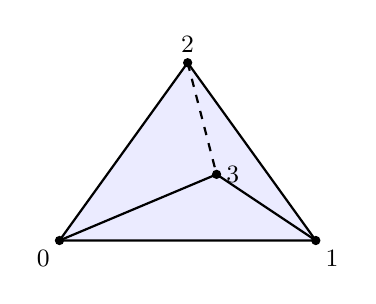
\begin{tikzpicture}[scale=1.05, every node/.style={font=\small}]
        \coordinate (v0) at (-1.55,-0.9);
        \coordinate (v1) at (1.55,-0.9);
        \coordinate (v2) at (0,1.25);
        \coordinate (v3) at (0.35,-0.1);

        \draw[fill=blue!8, draw=none] (v0) -- (v1) -- (v2) -- cycle;
        \draw[thick] (v0) -- (v1) -- (v2) -- cycle;
        \draw[thick] (v0) -- (v3);
        \draw[thick] (v1) -- (v3);
        \draw[thick,dashed] (v2) -- (v3);

        \fill (v0) circle (1.6pt) node[below left] {$0$};
        \fill (v1) circle (1.6pt) node[below right] {$1$};
        \fill (v2) circle (1.6pt) node[above] {$2$};
        \fill (v3) circle (1.6pt) node[right] {$3$};
    \end{tikzpicture}
    \end{center}
    Closing downward adds their edges and vertices. The geometric realization of this complex is homeomorphic to the surface of a sphere, or $S^2$. In that respect it is a \textit{triangulation} of $S^2$. 
\end{example}

Not all topological spaces are triangulable (i.e. have a simplicial complex to which they are homeomorphic), but many interesting ones are. Since we are only working with simplicial complexes we are only able to compute homology for spaces with triangulations, but there are more general notions of homology which apply to all topological spaces.  

\subsection{Homology}

Computing is one way of associating abelian groups to a simplicial complex in a way that gives us important information about their structure. The basic idea is to stop thinking about \textit{geometry} and instead think about formal sums of simplices and record how they meet along their faces. 

Let $K$ be a finite simplicial complex. For each $k\geq 0$, let $K_k$ denote the set of $k$-simplices of $K$. A \textbf{$k$-chain} is a formal integer linear combination of $k$-simplices. The set of all $k$-chains forms the free abelian group $C_k(K) \cong \mathbb Z^{K_k}$.

The next ingredient is the boundary operation. The \textbf{boundary} of a simplex is a formal sum of its codimension-one faces, with signs chosen so that repeated faces cancel when taking the boundary twice. If the vertices of an oriented simplex are ordered as $[v_0,v_1,\dots, v_k]$, then $$\partial_k[v_0,\dots,v_k] = \sum_{i=0}^k (-1)^i[v_0,\dots,\widehat{v_i},\dots, v_k]$$ where the hat means the vertex is omitted. For example, the boundary of an oriented edge $[a,b]$ is $[b]-[a]$ and the boundary of an oriented triangle $[a,b,c]$ is $[b,c]-[a,c] + [a,b]$. Extend this process linearly and we get a group homomorphism $$\partial_k : C_k(K) \to C_{k-1}(K)$$ called the \textbf{boundary map}. 

There are two special kinds of chains. A \textbf{$k$-cycle} is a $k$-chain whose boundary is equal to $0$. A \textbf{$k$-boundary} is a $k$-chain that is the boundary of some $(k+1)$-chain. It happens that for each $k$, $\partial_k\circ\partial_{k+1}=0$, which means that every boundary is a cycle. Algebraically, we have $\text{im }\partial_{k+1} \subseteq \text{ker }\partial_k$. Then we can define the \textbf{$k$th simplicial homology group} of $K$ as the quotient $$H_k(K;\mathbb Z) = \ker \partial_k / \operatorname{im}\partial_{k+1}.$$
 In a few words, homology keeps track of the cycles but thinks of two cycles as equivalent if they differ by a boundary. 

We can think of this as a matrix computation by choosing a basis for each chain group. A natural choice is the set of $k$-simplices, but we need to choose an ordering on this basis as well in order to keep the sign convention consistent. In ChainCert we assume the vertex type comes with a linear order, and takes the lexicographic order on $k$-simplices. With these bases fixed, we can think of each boundary map $\partial_k$ as a matrix of integers. 

\subsection{Using SNF to Compute Simplicial Homology}

Once bases for the chain groups are fixed, each boundary map is represented by
an integer matrix. Suppose that
\[
    \partial_k : \mathbb{Z}^{n_k} \to \mathbb{Z}^{n_{k-1}}
    \qquad\text{and}\qquad
    \partial_{k+1} : \mathbb{Z}^{n_{k+1}} \to \mathbb{Z}^{n_k}
\]
are the two consecutive boundary maps needed to compute $H_k$. The chain
condition says that
\[
    \partial_k \partial_{k+1} = 0,
\]
so every column of the matrix for $\partial_{k+1}$ lies in the kernel of
$\partial_k$.

The first step is to compute the Smith normal form of $\partial_k$. This puts
$\partial_k$ into diagonal form after changing bases in the domain and codomain.
If the diagonal has $r_k$ nonzero entries, then the kernel of $\partial_k$ is a
free abelian group of rank $n_k-r_k$. In the new domain basis, the last
$n_k-r_k$ basis vectors span the cycle group $\ker\partial_k$.

We must then understand the image of $\partial_{k+1}$ as a subgroup of this
cycle group. After applying the same change of basis to the columns of
$\partial_{k+1}$, the first $r_k$ coordinates vanish because
$\partial_k\partial_{k+1}=0$. The remaining $n_k-r_k$ rows form a matrix
\[
    M_k : \mathbb{Z}^{n_{k+1}} \to \mathbb{Z}^{n_k-r_k}
\]
whose image is exactly the boundary subgroup inside the cycle coordinates.
Therefore
\[
    H_k(K;\mathbb{Z})
      \cong \mathbb{Z}^{n_k-r_k} / \operatorname{im} M_k.
\]

Now \Cref{prop:snf-bridge} applies directly to the presentation matrix $M_k$.
If the Smith normal form of $M_k$ has nonzero diagonal entries
$d_1,\ldots,d_s$, then
\[
    H_k(K;\mathbb{Z})
      \cong \mathbb{Z}^{\,n_k-r_k-s}
          \oplus \bigoplus_{i : d_i \text{ is a non-unit}} \mathbb{Z}/d_i\mathbb{Z}.
\]
Over the integers, the non-unit diagonal entries are exactly the torsion
coefficients greater than $1$ up to sign, and the free rank
$n_k-r_k-s$ is the $k$-th Betti number.

This is the computation ChainCert certifies. Sage is used to find the Smith
normal forms, but Lean checks the resulting certificates, checks the chain
condition, constructs the presentation matrix $M_k$, and verifies that the final
read-off of the free rank and torsion coefficients follows from the certified
SNF data.

\section{Certificates}\label{sec:certificates}
\subsection{SNF Certificates}

The basic certificate in ChainCert is an SNF certificate for a matrix. Suppose
$A$ is an $m\times n$ matrix over a PID. Instead of asking Lean to compute the
Smith normal form of $A$, Sage returns the diagonal matrix $D$ together with
change-of-basis matrices $U$ and $V$ and their inverses. Lean then checks that
these matrices really witness a Smith normal form.

\begin{lstlisting}[caption={The core SNF certificate.},label={lst:snf-certificate}]
structure CertificateSNF (A : Matrix (Fin m) (Fin n) R) where
  U    : Matrix (Fin m) (Fin m) R
  Uinv : Matrix (Fin m) (Fin m) R
  V    : Matrix (Fin n) (Fin n) R
  Vinv : Matrix (Fin n) (Fin n) R
  D    : Matrix (Fin m) (Fin n) R
  r    : ℕ := firstZeroDiag D
  hrankCutoff : r = firstZeroDiag D                       := by native_decide
  hdiag  : IsDiagonal D                                   := by native_decide
  hrank  : ∀ i : Fin (min m n),
              diagEntry D i = 0 ↔ r ≤ i.val               := by native_decide
  hUUinv : U * Uinv = 1                                   := by native_decide
  hVVinv : V * Vinv = 1                                   := by native_decide
  heq    : U * A * V = D                                  := by native_decide
  hdiv   : divChainWithinRank D                           := by native_decide
\end{lstlisting}

The fields fall into three groups. The first group, \lean{U}, \lean{V}, and
\lean{D}, is the mathematical data of the Smith normal form. The field
\lean{heq} is the SNF identity itself: \(UAV = D\). The second group,
\lean{Uinv} and \lean{Vinv}, exists for verification efficiency. By
\Cref{def:snf}, the change-of-basis matrices are required to be unimodular,
meaning their determinants are units. Checking unimodularity by computing
determinants symbolically gets expensive fast in any reasonable matrix size,
so instead Sage hands us the explicit inverses, and Lean just checks the
matrix product \(U U^{-1} = 1\) (this is \lean{hUUinv}; the symmetric flip
\lean{Uinv * U = 1} follows automatically for square matrices over a
commutative ring, and is provided as a derived lemma \lean{hUinvU}). Same story
for \(V\).

The third group encodes the structural conditions on \(D\) itself.
\lean{IsDiagonal D} says that every off-diagonal entry of \(D\) is zero
(off-diagonal here means \(i \neq j\) as natural numbers, since \(D\) is
rectangular). \lean{hdiv} packages the divisibility chain
\(d_1 \mid d_2 \mid \cdots\) from \Cref{def:snf} through the predicate
\lean{divChainWithinRank D}, which asserts the divisibility only for
\emph{consecutive} indices (the full chain follows by transitivity) and
only within the rank prefix (\(j < \mathtt{firstZeroDiag}\ D\)), since the
trailing zeros impose no constraint. The indices \(i, j\) range over
\(\mathtt{Fin}(\min m\, n)\) because that is the length of the diagonal
of an \(m \times n\) matrix.

The remaining piece is the rank. The number \lean{r} is defined to be
\lean{firstZeroDiag D}, the smallest index where the diagonal of \(D\)
vanishes (or \(\min m\, n\) if it never does). The field \lean{hrankCutoff}
records this definitional equation explicitly so that downstream proofs can
treat \lean{r} as an opaque $\mathbb{N}$ and unfold only when needed. The field
\lean{hrank} then says \(d_i = 0\) iff \(r \leq i\), which is the precise
``zero-tail'' condition on a diagonal in Smith form: the diagonal entries are
nonzero strictly before \(r\) and zero from \(r\) onward. Combined with
\lean{hdiv}, this matches \Cref{def:snf} exactly.

All of these fields are decidable predicates or equations between concrete
finite matrices. This is the whole point of the certificate format: Sage may
have used any algorithm it likes to produce \(U\), \(V\), \(D\), and the
inverses, but the conditions Lean checks are purely about the resulting matrix
data, with no reference to how it was obtained.

In the current implementation, every check is discharged with
\lean{native_decide} (the default tactics shown in the listing). This is
convenient because the goals are all finite computations on concrete integer
matrices, but it is not quite the same trust story as a proof by kernel
reduction alone: \lean{native_decide} relies on Lean's native-code evaluator,
so in principle it trusts more of Lean's compiler and runtime. The intended
claim is therefore not that the implementation has Mathlib's smallest possible
trusted base, but that Sage is not trusted for correctness of the
mathematical result. Sage supplies candidate data; Lean checks the certificate
fields itself.

\subsection{Homology Certificates}

The homology certificate packages together the SNF data needed for one degree
of homology. Recall from \Cref{sec:background} that computing \(H_k\) requires
two SNFs --- one for \(d_k\), which identifies the cycle group, and one for
the resulting presentation matrix \(M\) of the boundary image inside cycles.
The certificate carries both, plus the gluing data that ties them together.

It is stated for two consecutive boundary matrices
\[
    d_k : \mathbb{Z}^{n} \to \mathbb{Z}^{m},
    \qquad
    d_{k+1} : \mathbb{Z}^{p} \to \mathbb{Z}^{n}.
\]

\begin{lstlisting}[caption={The chain quotient certificate.},label={lst:chain-quotient-certificate}]
structure ChainQuotientCert
    (dk  : Matrix (Fin m) (Fin n) R)
    (dk1 : Matrix (Fin n) (Fin p) R) where
  certK : CertificateSNF dk
  hCC   : dk * dk1 = 0
  M     : Matrix (Fin (n - certK.r)) (Fin p) R
  hM    : M = cyclePresentationMatrix certK dk1
  certM : CertificateSNF M
\end{lstlisting}

There are five fields, each playing a specific role.

The first field, \lean{certK}, is an SNF certificate for \(d_k\). This is what
gives Lean enough information to talk about the cycle group \(\ker d_k\) in a
concrete basis: as explained in \Cref{sec:background} and made precise in
\Cref{sec:theorems}, the bottom \(n - r\) coordinates of \(V^{-1}\) give a
basis for cycles, where \(r\) is the rank cutoff stored inside \lean{certK}.

The second field, \lean{hCC}, is the chain condition \(d_k d_{k+1} = 0\). It
is a single matrix equation and so is discharged by the same
\lean{native_decide} kind of check. Without it, the quotient
\(\ker d_k / \operatorname{im} d_{k+1}\) is not even defined as a Mathlib
module.

The third field, \lean{M}, is the \emph{presentation matrix} for the boundary
image, written in cycle coordinates. Its row index has length \(n - r\),
which is exactly the dimension of the cycle space in the certified basis, and
its column index is \(p\), the number of \((k+1)\)-cells. Concretely,
\lean{M} is the matrix whose cokernel will present \(H_k\).

The fourth field, \lean{hM}, is what makes \lean{M} honest. The function
\lean{cyclePresentationMatrix certK dk1} is defined in
\lean{ChainCert/Homology/Basic.lean} as
\[
    \mathtt{cyclePresentationMatrix\ certK\ dk1}
      \;=\; \mathtt{bottomRows}\, r\, \bigl(V^{-1} \cdot d_{k+1}\bigr),
\]
that is, take the product \(V^{-1} d_{k+1}\) and keep only the rows from index
\(r\) onward. The condition \lean{hM : M = cyclePresentationMatrix certK dk1}
forces \lean{M} to be exactly this matrix, computed from the SNF data and
\(d_{k+1}\). The reader might reasonably ask why \lean{M} is stored
separately at all, given that it is determined by the other fields. The reason
is purely operational: storing \lean{M} as its own field lets Sage hand it to
Lean as a concrete integer matrix, which then becomes the input to a second
SNF certificate. The equation \lean{hM} is the guard rail that prevents
\lean{M} from drifting away from what the cycle-coordinate definition says it
should be.

The fifth field, \lean{certM}, is an SNF certificate for that presentation
matrix \(M\). This is the second SNF needed to read off Betti numbers and
torsion --- once Lean knows that \(H_k\) is the cokernel of \(M\) (the content
of \Cref{sec:theorems}), \lean{certM} reduces this further to the cokernel of
a diagonal matrix.

The certificate \lean{ChainQuotientCert} is deliberately stated independently
of simplicial complexes: it is a certificate for the quotient
\(\ker d_k / \operatorname{im} d_{k+1}\) associated to any two composable
matrices over a PID. The wrapper \lean{CertificateHomology} specializes this
to the boundary matrices of a finite facet complex:

\begin{lstlisting}[caption={The homology certificate for a finite facet complex.},label={lst:homology-certificate}]
structure CertificateHomology (X : FFC V) (k : ℕ) where
  quotientCert :
    ChainQuotientCert (boundaryK X k) (boundaryK X (k + 1))
\end{lstlisting}

This separation is useful because the algebraic verification of the quotient
does not depend on how the boundary matrices were produced. Any other source
of two composable integer matrices over \(\mathbb{Z}\) --- not just
simplicial boundary maps --- could plug into \lean{ChainQuotientCert} and
inherit the bridge theorems of \Cref{sec:theorems} verbatim.

\section{Theorems}\label{sec:theorems}

The point of a certificate is that the fields are tiny, finite-matrix checks,
but the conclusion is a statement about honest Mathlib submodules and
quotients. \Cref{sec:background} already explained \emph{how} one computes
homology from two SNFs; this section explains what ChainCert actually
\emph{proves} about that recipe. The bridge layer turns each step of the
algorithm into a linear equivalence between the certified matrix data and the
corresponding piece of Mathlib linear algebra, and then composes them.

Throughout, fix an SNF certificate \lean{cert : CertificateSNF A} for a matrix
\(A : \mathbb{Z}^n \to \mathbb{Z}^m\). We write \lean{matRange A} for the image
of the associated linear map.

\subsection{The SNF Bridge}

The first bridge says that the change-of-basis matrix \(U\) really is a linear
equivalence of \(\mathbb{Z}^m\), and that it carries the image of \(A\) onto
the image of the diagonal form \(D\). Concretely, \lean{rowLinearEquiv cert} is
the map \(x \mapsto U x\); it is invertible because the certificate carries
both \lean{U * Uinv = 1} and \lean{Uinv * U = 1}.

The range identity is the substantive statement. Given \(y = A z\) in the image
of \(A\), the certificate equation \(UAV = D\) lets us rewrite
\[
    U y \;=\; U(Az) \;=\; (UAV)(V^{-1}z) \;=\; D(V^{-1}z),
\]
so \(Uy\) is in the image of \(D\). The same computation read backwards, using
\(V V^{-1} = 1\), shows that every \(Dz'\) equals \(U(A(Vz'))\). Hence
\(U\) maps \(\operatorname{im}A\) bijectively onto \(\operatorname{im}D\).
Because \(U\) is a linear equivalence carrying one submodule onto another, it
descends to an equivalence of quotients:

\begin{lstlisting}[caption={The certified diagonal presents the same cokernel.},label={lst:cokernel-equivalence}]
noncomputable def cokernelEquivDiagonal (cert : CertificateSNF A) :
    ((Fin m → R) ⧸ matRange A) ≃ₗ[R]
      ((Fin m → R) ⧸ matRange cert.D)
\end{lstlisting}

This is exactly the cokernel side of the structure theorem
(\Cref{prop:snf-bridge}) made into a concrete linear equivalence: any module
presented by \(A\) is presented equally well by its certified diagonal form,
and the diagonal form is what we will read invariants from later.

\subsection{Cycles in Certified Coordinates}

For the homology bridge, fix two consecutive boundary matrices
\(d_k : \mathbb{Z}^n \to \mathbb{Z}^m\) and
\(d_{k+1} : \mathbb{Z}^p \to \mathbb{Z}^n\) with \(d_k d_{k+1} = 0\), and an
SNF certificate \lean{certK} for \(d_k\) with rank cutoff \(r\) (the index of
the first zero on the diagonal of the certified \(D\)).

The chain condition is essentially trivial to state and prove:
\(d_k d_{k+1} = 0\) immediately gives
\(\operatorname{im} d_{k+1} \subseteq \ker d_k\), so the homology quotient
\(\ker d_k / \operatorname{im} d_{k+1}\) is a well-defined Mathlib quotient
module (which the file calls \lean{matrixHomology dk dk1 hCC}).

The first real content is the \emph{cycle-coordinate equivalence}. The picture
from \Cref{sec:background} was: change basis in the domain of \(d_k\) by
\(V^{-1}\), and the kernel becomes the subspace of vectors whose first \(r\)
coordinates vanish, with the remaining \(n - r\) coordinates free. ChainCert
proves this directly. For any cycle \(x \in \ker d_k\),
\[
    D \cdot (V^{-1} x)
      \;=\; (UAV)\,(V^{-1} x)
      \;=\; U \cdot (d_k \, x)
      \;=\; 0.
\]
For each index \(j < r\), the \(j\)th diagonal entry of \(D\) is a unit (by
\lean{certK.hrank}, the diagonal is zero exactly past \(r\)), so the \(j\)th
coordinate of \(V^{-1} x\) must itself vanish. Thus \(V^{-1}\) sends a cycle to
a vector supported on coordinates \(r, r+1, \ldots, n - 1\), and the
``bottom \(n - r\) coordinates'' carry all the data. This is
\lean{cycleCoordinateEquiv certK}: the forward map sends \(x\) to
\(\mathtt{bottomCoordinates}(V^{-1} x)\), and the inverse extends a vector by
zeros on the top \(r\) coordinates and applies \(V\). The two compositions
collapse using \(V V^{-1} = V^{-1} V = 1\) together with the vanishing of
the top coordinates on cycles.

\subsection{The Presentation Matrix}

With the cycle-coordinate equivalence in hand, the only thing left is to write
\(\operatorname{im} d_{k+1}\) inside the cycle coordinates. The certificate
stores a matrix \lean{M} and a proof that
\[
    \mathtt{M} \;=\; \mathtt{cyclePresentationMatrix\ certK\ dk1}
        \;=\; \mathtt{bottomRows}\, r\, \bigl(V^{-1} \cdot d_{k+1}\bigr),
\]
i.e.\ \(M\) is the bottom \(n - r\) rows of \(V^{-1} d_{k+1}\). The
identification is then a one-line matrix computation: for any
\(z \in \mathbb{Z}^p\), the chain \(d_{k+1} z\) is a cycle, and its image
under the cycle-coordinate equivalence is
\begin{align*}
    \mathtt{bottomCoordinates}\bigl(V^{-1} (d_{k+1} z)\bigr)
      &\;=\; \mathtt{bottomCoordinates}\bigl((V^{-1} d_{k+1})\, z\bigr) \\
      &\;=\; \bigl(\mathtt{bottomRows}\, r\,(V^{-1} d_{k+1})\bigr)\, z
       \;=\; M z.
\end{align*}
So as \(z\) ranges over \(\mathbb{Z}^p\), the image of
\(\operatorname{im} d_{k+1}\) under the cycle-coordinate equivalence traces
out exactly \(\operatorname{im} M\). This is
\lean{map_boundaryImage_eq_presentationRange}, the central bookkeeping lemma
of the homology bridge: \(M\) is not an auxiliary object, it is the next
boundary map written in the certified basis for cycles.

Quotienting by equal submodules across an equivalence then gives a linear
equivalence
\[
    \ker d_k / \operatorname{im} d_{k+1}
      \;\cong\; \mathbb{Z}^{n - r} / \operatorname{im} M,
\]
formalized as \lean{ChainQuotientCert.homologyEquivPresentation}.

\subsection{Composing the Two Bridges}

At this point, the homology of \((d_k, d_{k+1})\) has been identified with the
cokernel of a single matrix \(M\), so the SNF bridge of
\Cref{sec:certificates} applies to \(M\) directly. The certificate stores an
SNF certificate \lean{certM} for \(M\), and composing the two equivalences
gives the headline statement:

\begin{lstlisting}[caption={The final homology bridge.},label={lst:homology-diagonal-equivalence}]
noncomputable def homologyEquivDiagonal
    (cert : CertificateHomology X k) :
    cert.homologyModule ≃ₗ[R]
      ((Fin (cellCount X k - cert.quotientCert.certK.r) → R) ⧸
        matRange cert.presentationCert.D)
\end{lstlisting}

This says: the actual algebraic homology group
\(H_k(X;\mathbb{Z})\), in the form \(\ker \partial_k / \operatorname{im}
\partial_{k+1}\), is linearly equivalent to the cokernel of an explicit
diagonal integer matrix, whose entries Lean has separately verified to be the
Smith normal form of the presentation matrix \(M\). Combined with
\Cref{prop:snf-bridge}, this is the formal endpoint of the recipe of
\Cref{sec:background}: the Betti number and torsion coefficients of \(H_k\)
can now be read off from a diagonal matrix that lives entirely in checked Lean
data.

\section{Tactics and Commands}\label{sec:tactics}

ChainCert exposes the Sage bridge through two kinds of interface. Commands such
as \lean{#snf} and \lean{#homology} are exploratory: they ask Sage for a result
and print it in the Lean infoview. Tactics such as \lean{snf} and
\lean{homology} are proof-producing: they call Sage for candidate data, rebuild
that data as Lean expressions, and construct certificates that Lean checks.

\subsection{The \texttt{snf} Tactic}

The \lean{snf} tactic computes a Smith normal form certificate for a concrete
matrix. The basic syntax is:

\begin{lstlisting}[caption={Using the \texttt{snf} tactic.},label={lst:snf-tactic}]
example : True := by
  snf A
  -- cert : CertificateSNF A
  trivial

example : True := by
  snf A as hA
  -- hA : CertificateSNF A
  trivial
\end{lstlisting}

The tactic is goal-agnostic: it adds a certificate to the local context and
leaves the current goal unchanged. Internally, it serializes the entries of
\lean{A}, sends the matrix to Sage, receives matrices \lean{U}, \lean{Uinv},
\lean{D}, \lean{V}, and \lean{Vinv}, and reconstructs a term of type
\lean{CertificateSNF A}. Lean then checks the fields of the certificate by
finite matrix computation, in the current implementation usually through
\lean{native_decide}.

The matrix must have type \lean{Matrix (Fin m) (Fin n) R}, and its entries must
be serializable to Sage. The tactic is intended for concrete matrices whose
entries can be evaluated during elaboration; fully symbolic matrices are not
sent to Sage.

Serialization is handled by the typeclass \lean{SageSerializable}. An instance
specifies how to print elements of a Lean type as Sage-readable strings, how to
parse Sage's string output back into Lean, and the name of the corresponding
Sage ring. The project currently provides instances for \(\mathbb{Z}\) and
\(\mathbb{Q}\). This is an implementation constraint, not a mathematical one:
even if a coefficient ring is a PID in Lean, these Sage-backed tactics can use
it only after a \lean{SageSerializable} instance explains how to translate its
elements to and from Sage. For example:

\begin{lstlisting}[caption={The serialization interface for coefficient rings.},label={lst:sage-serializable}]
class SageSerializable (R : Type*) where
  toSageString   : R → String
  fromSageString : String → Option R
  sageName       : String
\end{lstlisting}

This typeclass is deliberately small. Sage's output is not trusted merely
because it parses successfully; parsing only reconstructs candidate matrices.
The certificate fields are still checked in Lean afterward.

\subsection{The \texttt{homology} Tactic}

The \lean{homology} tactic computes a certified homology presentation for a
finite facet complex in one degree. In the examples below,
\lean{triangleFFC} is the finite facet complex on vertices \lean{Fin 3} with a
single facet \(\{0,1,2\}\). In other words, it is the filled triangle
2-simplex, not just its boundary cycle. The syntax mirrors the \lean{snf}
tactic:

\begin{lstlisting}[caption={Using the \texttt{homology} tactic.},label={lst:homology-tactic}]
example : True := by
  homology triangleFFC, 1
  -- homologyCert : CertificateHomology triangleFFC 1
  trivial

example : True := by
  homology triangleFFC, 1 as hTri
  -- hTri : CertificateHomology triangleFFC 1
  trivial

example : CertificateHomology triangleFFC 1 := by
  homology triangleFFC, 1
\end{lstlisting}

When the current goal is already the matching \lean{CertificateHomology} type,
the tactic closes the goal. Otherwise it adds a certificate to the context. The
certificate contains the SNF certificate for the boundary matrix
\(\partial_k\), the checked chain condition
\(\partial_k\partial_{k+1}=0\), the cycle-presentation matrix, and an SNF
certificate for that presentation matrix.

\subsection{Exploratory Commands}

The commands are useful for inspecting Sage output while developing examples.
The command \lean{#snf A} prints the raw SNF data returned by Sage, and
\lean{#homology X, k} prints the homology group Sage computes for the finite
facet complex \lean{X} in degree \lean{k}. These commands are intentionally not
the trusted interface: the trusted path is through the tactics, which turn the
Sage output into Lean-checked certificates.

\section{Examples}\label{sec:examples}

This section walks through three uses of the \lean{homology} pipeline,
ordered by increasing complexity. The first two are landed and
kernel-checked in \texttt{ChainCert.Examples}; the third is a target that
exposes the current limits of the implementation and motivates the
discussion in \Cref{sec:future-work}.

\subsection{The Triangle: \texorpdfstring{$H_1(\Delta^2;\mathbb{Z})=0$}{H1(Triangle)=0}}

The filled \(2\)-simplex \lean{triangleFFC} on three vertices is the
smallest non-trivial finite facet complex. Its first homology vanishes
because the unique boundary \(\partial_2(\{0,1,2\})\) generates the entire
cycle group of the triangle. The Sage--Lean pipeline reproduces this in
two steps.

First, the \lean{homology} tactic produces a Sage-checked certificate:
\begin{lstlisting}[caption={Triangle $H_1$ certificate.},label={lst:triangle-cert}]
noncomputable def triangleH1Cert :
    CertificateHomology (R := ℤ) triangleFFC 1 := by
  homology triangleFFC, 1
\end{lstlisting}

Second, the \texttt{homologyEquivPi} bridge identifies the abstract
homology module with a product of row-ideal quotients of the certified
diagonal Smith form \(D\). For the triangle the presentation matrix has
SNF \(\operatorname{diag}(1)\), so the single factor is
\(\mathbb{Z}\,/\,\langle 1\rangle = 0\):

\begin{lstlisting}[caption={The certified $H_1$ of the triangle is trivial.},label={lst:triangle-subsingleton}]
theorem triangleH1_subsingleton :
    Subsingleton triangleH1Cert.homologyModule
\end{lstlisting}

The proof is \texttt{native\_decide} on the diagonal entries of the
certificate's Smith form, combined with the general fact that a row-ideal
quotient \(\mathbb{Z}\,/\,\langle u\rangle\) is trivial whenever \(u\) is a
unit.

\subsection{The Projective Plane: \texorpdfstring{$H_1(\mathbb{R}P^2;\mathbb{Z})=\mathbb{Z}/2\mathbb{Z}$}{H1(RP2)=Z/2Z}}

The real projective plane is the smallest closed surface whose integral
homology has torsion. The minimal triangulation
\lean{rp2FFC} on six vertices has 15 edges and 10 triangles; each edge
appears in exactly two triangles and \(V-E+F = 6-15+10 = 1 = \chi(\mathbb{R}P^2)\).
The certificate is built the same way as for the triangle:

\begin{lstlisting}[caption={$\mathbb{R}P^2$ $H_1$ certificate (Sage-backed).},label={lst:rp2-cert}]
noncomputable def rp2H1Cert :
    CertificateHomology (R := ℤ) rp2FFC 1 := by
  homology rp2FFC, 1
\end{lstlisting}

The composition \texttt{homologyEquivDiagonal} of \Cref{lst:homology-diagonal-equivalence}
specialises to give the headline correctness statement for this example:

\begin{lstlisting}[caption={$\mathbb{R}P^2$: certified homology equals the cokernel of the Sage diagonal.},label={lst:rp2-bridge}]
theorem rp2H1_equiv_sage_diagonal_pi :
    Nonempty (rp2H1Cert.homologyModule ≃ₗ[ℤ]
      ∀ i : Fin (cellCount rp2FFC 1 - rp2H1Cert.quotientCert.certK.r),
        ℤ ⧸ rowDiagIdeal (R := ℤ) rp2H1Cert.presentationCert.D i)
\end{lstlisting}

This is precisely the statement promised by the bridge of
\Cref{sec:theorems}: the abstract homology module of the simplicial
complex is linearly equivalent to the cokernel of the integer diagonal
matrix returned by Sage. The remaining question is which diagonal Sage
actually returned. Three short \texttt{native\_decide} probes pin it
down:

\begin{lstlisting}[caption={Structural facts about the certified Smith diagonal for $\mathbb{R}P^2$.},label={lst:rp2-torsion-structure}]
theorem rp2_presentation_size :
    cellCount rp2FFC 1 - rp2H1Cert.quotientCert.certK.r = 10

theorem rp2_unique_non_unit_diagonal :
    (Finset.univ.filter (fun i =>
        ¬ IsUnit (rowDiagVal rp2H1Cert.presentationCert.D i))).card = 1

theorem rp2_torsion_diagonal_is_two
    (i) (hi : ¬ IsUnit (rowDiagVal rp2H1Cert.presentationCert.D i)) :
    (rowDiagVal rp2H1Cert.presentationCert.D i).natAbs = 2
\end{lstlisting}

Together with \Cref{lst:rp2-bridge}, these three statements say: the
certified homology of \(\mathbb{R}P^2\) in degree \(1\) is isomorphic to a
product of ten row-ideal quotients of \(\mathbb{Z}\); nine of those
factors are quotients by units (hence trivial); the remaining factor is a
quotient by an integer of absolute value \(2\) (hence \(\mathbb{Z}/2\mathbb{Z}\)).
The classical answer \(H_1(\mathbb{R}P^2;\mathbb{Z})=\mathbb{Z}/2\mathbb{Z}\)
is thereby recovered as a corollary of the bridge plus three small
kernel-checked computations on Sage output.

\subsection{The Klein Bottle: A Current Limit}\label{sec:klein-attempt}

The Klein bottle is the natural next example. The intended target is
\(H_0(K;\mathbb{Z}) \cong \mathbb{Z}\),
\(H_1(K;\mathbb{Z}) \cong \mathbb{Z} \oplus \mathbb{Z}/2\mathbb{Z}\), and
\(H_2(K;\mathbb{Z}) = 0\). We have a triangulation
\lean{kleinBottleFFC} on nine vertices with eighteen triangles ready in
\texttt{ChainCert.Examples.Complexes}, and Sage returns the expected
Smith data in well under a second. The certificate, however, currently
does not close in the Lean kernel:
\begin{lstlisting}[caption={Klein bottle: cert still has a heartbeat-bound \texttt{sorry}.},label={lst:klein-attempt}]
set_option maxHeartbeats 4000000 in
noncomputable def kleinBottleH1Cert :
    CertificateHomology (R := ℤ) kleinBottleFFC 1 := by
  homology kleinBottleFFC, 1   -- exceeds heartbeats
\end{lstlisting}
The bottleneck is the chain-condition obligation
\(\partial_1 \partial_2 = 0\), which the \lean{homology} tactic discharges
by \texttt{native\_decide} on a matrix product. On nine vertices and
eighteen triangles this exhausts the configured heartbeat budget even at
\texttt{maxHeartbeats 4000000}. The example is therefore parked behind a
comment in \texttt{ChainCert.Examples.KleinBottleHomology}; the obstacle
is implementation, not mathematics, and the remediation paths are
discussed below.

\section{Future Work}\label{sec:future-work}

The bridge of \Cref{sec:theorems} and its specialisation to \(\mathbb{R}P^2\)
in \Cref{sec:examples} together establish the main correctness statement
of this project: the certified homology module of a finite facet complex
is linearly equivalent to the cokernel of the integer diagonal matrix
returned by Sage. There are nevertheless several items the present
implementation does \emph{not} discharge, and which are useful to make
explicit before listing them as forward work.

\begin{itemize}
\item The Klein bottle certificate does not close: the \lean{homology}
tactic's chain-condition obligation exceeds the kernel heartbeat budget
(see \Cref{sec:klein-attempt}).
\item There is no Lean object bundling \(\{\partial_k\}_k\) into a
\lean{ChainComplex (ModuleCat ℤ) ℕ}, and consequently no theorem
connecting the certified \lean{homologyModule} to Mathlib's homology
of a chain complex.
\item For \(\mathbb{R}P^2\), the writeup pins down
\(H_1\cong\mathbb{Z}/2\mathbb{Z}\) through three structural facts
(\Cref{lst:rp2-torsion-structure}), but does not exhibit an explicit
linear equivalence \lean{homologyModule} \(\simeq_\ell\) \lean{ZMod 2}.
\item The \lean{homology} tactic is specialised to \(\mathbb{Z}\) through
the \lean{SageSerializable} instance, even though the certificate types
are generic in the coefficient ring.
\end{itemize}

The paragraphs below describe the route forward for each.

\paragraph{Heartbeat-bound examples.}
The Klein-bottle obstruction of \Cref{sec:klein-attempt} is the most
immediate item. Two routes are open. The first is a once-and-for-all
structural proof that \(\partial_k\partial_{k+1} = 0\) holds for any
simplicial chain complex over \(\mathbb{Z}\); this would replace the
per-example \texttt{native\_decide} on a matrix product with a single
kernel-friendly lemma, and would simultaneously unlock arbitrarily large
triangulations. The second is a smarter proof-by-reflection of matrix
product equality that works in blocks, trading kernel time for a slightly
more involved tactic. Either suffices for Klein bottle and related
medium-scale surfaces.

\paragraph{Bridging to \texttt{HomologicalComplex}.}
The bridge theorems of \Cref{sec:theorems} identify the algebraic quotient
\(\ker\partial_k / \operatorname{im}\partial_{k+1}\), expressed in matrix
coordinates, with the cokernel of the Sage-certified diagonal Smith form.
What they do not yet do is connect this to Mathlib's
\lean{HomologicalComplex.homology}: there is no Lean object yet that
bundles the family \(\{\partial_k\}_k\) of boundary matrices for a finite
facet complex into a \lean{ChainComplex (ModuleCat ℤ) ℕ}. Producing such
an object and proving the equivalence
\lean{(FFC.chainComplex X).homology k} \(\simeq_{\ell}\)
\lean{cert.homologyModule}
would let downstream users plug ChainCert certificates into the rest of
the categorical homological algebra in Mathlib. The main missing
ingredient is the same \(\partial^2 = 0\) lemma identified above.

\paragraph{Coefficients beyond \(\mathbb{Z}\).}
The certificate types are generic in the coefficient ring \(R\), but the
\lean{homology} tactic currently runs Sage's SNF over \(\mathbb{Z}\)
through the \lean{SageSerializable} instance for integers. The
serialization layer is already general enough to extend to \(\mathbb{Q}\)
(which is supported) and any other ring that admits a Sage round-trip; the
work is to wire the relevant Sage SNF backends and adjust the \lean{snf}
tactic to dispatch on the coefficient ring.

\paragraph{Explicit \(\mathrm{ZMod}\) decomposition.}
For \(\mathbb{R}P^2\) the writeup pins down
\(H_1\cong\mathbb{Z}/2\mathbb{Z}\) via the three structural facts of
\Cref{lst:rp2-torsion-structure}. A general utility lemma
\(\prod_i \mathbb{Z}/\langle a_i\rangle \simeq_\ell \prod_i
\mathrm{ZMod}\,|a_i|\), specialising the existing
\lean{quotientDiagonalEquivPiZMod} skeleton in
\texttt{ChainCert/Later/SNFQuotient.lean}, would let one read off
\(H_k(X;\mathbb{Z})\) as a concrete product of \lean{ZMod n} factors
directly from the Sage diagonal.

\section*{Acknowledgments}
The Lean-side Sage transport layer (the persistent subprocess wrapper in \texttt{SageServer.lean}) is adapted from earlier Lean--Sage tactic infrastructure by M.~Karatarakis. The original source is attributed in the file header in the project source.

%\section{Mathematical Background}

%\begin{definition}[Example definition]\label{def:example}
%Let $X$ be a set\ldots
%\end{definition}

%\begin{theorem}[Main result]\label{thm:main}
%For every $n \in \mathbb{N}$, the following holds: $\sum_{k=1}^{n} k = \frac{n(n+1)}{2}$.
%\end{theorem}

%\begin{proof}
%By induction on $n$. The base case is immediate. For the inductive step\ldots
%\end{proof}

%\section{Formalization in Lean}

%The Lean statement corresponding to \Cref{thm:main} is shown below.

%\begin{lstlisting}[caption={Statement of the main theorem.},label={lst:main}]
%theorem sum_range_succ (n : ℕ) :
%    ∑ k in Finset.range (n + 1), k = n * (n + 1) / 2 := by
%  induction n with
%  | zero => simp
%  | succ n ih =>
%    rw [Finset.sum_range_succ, ih]
%    ring
%\end{lstlisting}

%Inline references like \lean{Finset.range} work too.

\bibliographystyle{plain} \bibliography{refs}

\end{document}
